\documentclass[tikz,border=1mm]{standalone}
\usepackage{pgfgantt}
\usepackage{amsfonts,amsmath,amssymb,pifont}
\usetikzlibrary{positioning,arrows,shadows,shapes.symbols,shapes.geometric}
\usepackage{soul} % for highlights
\renewcommand{\familydefault}{\sfdefault}

% colors
\definecolor{myblue}{rgb}{0.4, 0.6, 0.8}
\definecolor{mycoral}{rgb}{0.97,0.51,0.47}
\definecolor{mygreen}{rgb}{0.66,0.89,0.63}
\definecolor{myocra}{rgb}{1, 0.8, 0.4}
\definecolor{mypurple}{rgb}{0.7, 0.6, 0.9}


% arrows
\tikzset{
  line/.style={
    draw, -latex', thick, rounded corners=3mm,
  }
}


% bar for work package
\newganttchartelement{package}{
package/.style={shape=signal, draw=black, drop shadow, signal pointer angle=120},
package height=1,
package top shift=-0.01pt,
package left shift=-0.15pt,
package right shift=-0.3pt
}


% bar for task
\newganttchartelement{task}{
task/.style={drop shadow, draw=black, rounded corners=3pt},
task height=1,
task top shift=-0.01pt
%task top shift=0.05pt
}

% deliverables
\newganttchartelement*{deliver}{
deliver/.style={shape=circle, draw=black, scale=0.4},
deliver height=1,
%deliver left shift=1pt,
deliver top shift=-0.01pt
}

% background lines
\tikzset{
   hline/.style={
        line width=\ganttvalueof{y unit chart},
        yshift=-0.5*\ganttvalueof{y unit chart},
        opacity=0.3
   },
   vline/.style={
   	line width=\ganttvalueof{x unit},
        opacity=0.2
   }
}


\begin{document}
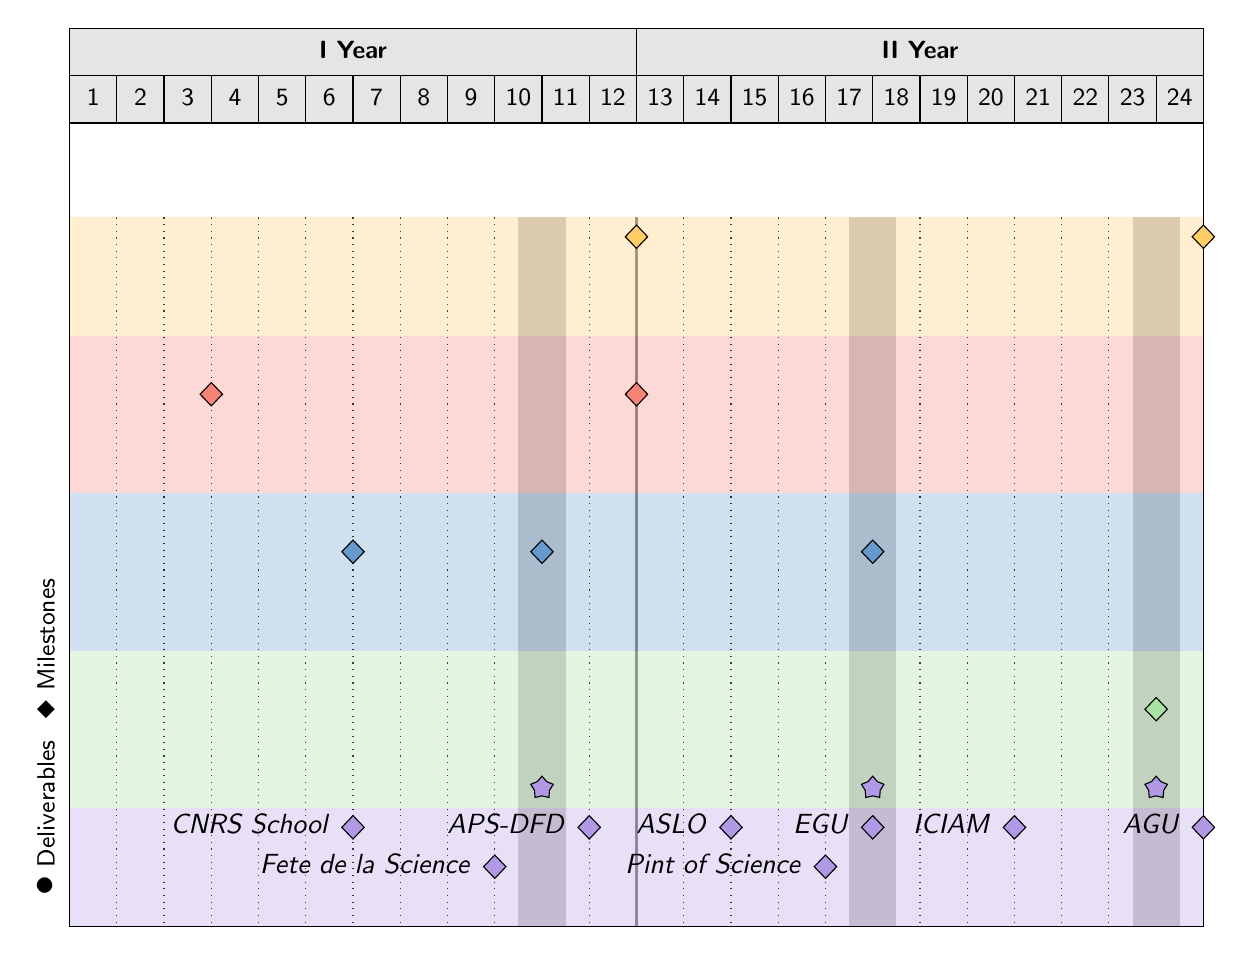
\begin{tikzpicture}[font=\small]
\begin{ganttchart}[
x unit = 0.6cm,
y unit chart = 0.5cm,
y unit title = 0.6cm,
hgrid={*3{hline,myocra},*4{hline,mycoral},*4{hline,myblue},*4{hline,mygreen},*5{hline,mypurple}},
vgrid={*9{dotted},*1{vline, black},*1{dotted},*1{solid, gray, thick},*4{dotted},*1{vline,black},*5{dotted},*1{vline, black}},
milestone height=1,
milestone inline label node/.append style={left=2mm},
milestone/.style={shape=diamond, draw=black, scale=0.6},
milestone top shift=-0.01pt,
title/.append style={shape=rectangle, fill=gray!20}, 
title height=1,
inline
]{1}{24}


% title
\gantttitle{\bf I Year}{12}
\gantttitle{\bf II Year}{12}\\
\gantttitlelist{1,...,24}{1}\\


% WP1: Management
\sethlcolor{myocra}
\ganttpackage[package/.append style={fill=myocra}]{\bf WP1}{1}{24}\\
% meetings
\ganttdeliver[deliver/.append style={fill=myocra}]{}{3}
\ganttdeliver[deliver/.append style={fill=myocra}]{}{6}
\ganttdeliver[deliver/.append style={fill=myocra}]{}{9}
\ganttdeliver[deliver/.append style={fill=myocra}]{}{12}
\ganttdeliver[deliver/.append style={fill=myocra}]{}{15}
\ganttdeliver[deliver/.append style={fill=myocra}]{}{18}
\ganttdeliver[deliver/.append style={fill=myocra}]{}{21}
\ganttdeliver[deliver/.append style={fill=myocra}]{}{24}\\
% reports
\ganttmilestone[milestone/.append style={fill=myocra}]{}{12}
\ganttmilestone[milestone/.append style={fill=myocra}]{}{24}\\


% WP2: Models
\ganttpackage[package/.append style={fill=mycoral!60}]{\bf WP2}{1}{12}\\
\gantttask[name=deriv, task/.append style={fill=mycoral}]{T2.1}{1}{3}
\gantttask[name=toy, task/.append style={fill=mycoral}]{T2.2}{4}{12}\\
\ganttdeliver[deliver/.append style={fill=mycoral}]{}{2}
\ganttdeliver[deliver/.append style={fill=mycoral}]{}{3}\\
\ganttmilestone[milestone/.append style={fill=mycoral}]{}{3}
\ganttmilestone[milestone/.append style={fill=mycoral}]{}{12}\\

% WP3: Simulations
\ganttpackage[package/.append style={fill=myblue!60}]{\bf WP3}{4}{17}\\
\gantttask[name=dns0, task/.append style={fill=myblue}]{T3.1}{4}{6}
\gantttask[name=dns1, task/.append style={fill=myblue}]{T3.2}{7}{10}
\gantttask[name=dns2, task/.append style={fill=myblue}]{T3.3}{11}{17}\\
\ganttdeliver[deliver/.append style={fill=myblue}]{}{5}
\ganttdeliver[deliver/.append style={fill=myblue}]{}{8}\\
\ganttmilestone[milestone/.append style={fill=myblue}]{}{6}
\ganttmilestone[milestone/.append style={fill=myblue}]{}{10}
\ganttmilestone[milestone/.append style={fill=myblue}]{}{17}\\

% WP4: Applications
\ganttpackage[package/.append style={fill=mygreen!60}]{\bf WP4}{18}{23}\\
\gantttask[name=exp, task/.append style={fill=mygreen}]{T4.1 \& T4.2}{18}{23}\\
\ganttdeliver[deliver/.append style={fill=mygreen}]{}{20}\\
\ganttmilestone[milestone/.append style={fill=mygreen}]{}{23}\\


% WP5: Dissemination
\ganttpackage[package/.append style={fill=mypurple}]{\bf WP5}{1}{24}\\
% scientific publications
\ganttmilestone[milestone/.append style={shape=star, fill=mypurple}]{}{10}
\ganttmilestone[milestone/.append style={shape=star, fill=mypurple}]{}{17}
\ganttmilestone[milestone/.append style={shape=star, fill=mypurple}]{}{23}\\
% conferences
% ICIAM: Tokyo August 2023 (every 4 year)
% ETC: Aug-Sept 2021 / 2023
% AGU Fall Meeting: December (every year)
% EGU Meeting: April/May (every year)
% Ocean Sciences Meeting: February-March 2022,2024
% APS-DFD: November (every year)
\ganttmilestone[milestone/.append style={shape=diamond, fill=mypurple}]{CNRS School}{6}
\ganttmilestone[milestone/.append style={shape=diamond, fill=mypurple}]{APS-DFD}{11}
\ganttmilestone[milestone/.append style={shape=diamond, fill=mypurple}]{ASLO}{14}
\ganttmilestone[milestone/.append style={shape=diamond, fill=mypurple}]{EGU}{17}
\ganttmilestone[milestone/.append style={shape=diamond, fill=mypurple}]{ICIAM}{20}
\ganttmilestone[milestone/.append style={shape=diamond, fill=mypurple}]{AGU}{24}\\
% outreach
\ganttmilestone[milestone/.append style={shape=diamond, fill=mypurple}]{Fete de la Science}{9}
\ganttmilestone[milestone/.append style={shape=diamond, fill=mypurple}]{Pint of Science}{16}\\


\end{ganttchart}


% Legend
\node at (-0.3,-9.0)[align=left, rotate=90] {{\Large $\bullet$} Deliverables $\,$ \ding{117} Milestones};


\end{tikzpicture}
\end{document}